%; whizzy document
% latex beamer presentation.
% platex, latex-beamer でコンパイルすることを想定。 

%     Tokyo Debian Meeting resources
%     Copyright (C) 2006 Junichi Uekawa

%     This program is free software; you can redistribute it and/or modify
%     it under the terms of the GNU General Public License as published by
%     the Free Software Foundation; either version 2 of the License, or
%     (at your option) any later version.

%     This program is distributed in the hope that it will be useful,
%     but WITHOUT ANY WARRANTY; without even the implied warranty of
%     MERCHANTABILITY or FITNESS FOR A PARTICULAR PURPOSE.  See the
%     GNU General Public License for more details.

%     You should have received a copy of the GNU General Public License
%     along with this program; if not, write to the Free Software
%     Foundation, Inc., 51 Franklin St, Fifth Floor, Boston, MA  02110-1301 USA

% 実行順番
% sudo  ~/bin/usb-macbook-ir.c &
% real presentation (shell-command (concat "DISPLAY=:0.1 xpdf -fullscreen " (replace-regexp-in-string "tex$" "pdf"(buffer-file-name)) "&"))
% DISPLAY=:0.1 xpdf -fullscreen 

\documentclass[cjk,dvipdfmx,14pt]{beamer}
% 14 seems like the max relevant value 
\usetheme{Warsaw}
\usepackage{fancybox}%SBox

%  preview (shell-command (concat "xpdf " (replace-regexp-in-string "tex$" "pdf"(buffer-file-name)) "&"))
%  presentation (shell-command (concat "xpdf -fullscreen " (replace-regexp-in-string "tex$" "pdf"(buffer-file-name)) "&"))


%http://www.naney.org/diki/dk/hyperref.html
%日本語EUC系環境の時
\AtBeginDvi{\special{pdf:tounicode EUC-UCS2}}
%シフトJIS系環境の時
%\AtBeginDvi{\special{pdf:tounicode 90ms-RKSJ-UCS2}}

\title{真のLinux Kernel 向けシェル}
\subtitle{LL GONG @ LL RING 2006}
\author{上川 純一 \\dancer@debian.org\\ Debian Project}
\date{2006年8月26日}
\logo{
\includegraphics[width=8cm]{image200607/openlogo-light.eps}}

% 三択問題用
\newcounter{santakucounter}
\newcommand{\santaku}[5]{%
\addtocounter{santakucounter}{1}
\frame{\frametitle{問題\arabic{santakucounter}. #1}
%問題\arabic{santakucounter}. #1
\begin{minipage}[t]{0.7\hsize}
 \begin{itemize}
 \item A #2\\
 \item B #3\\
 \item C #4\\
 \end{itemize}
\end{minipage}
}
\frame{\frametitle{問題\arabic{santakucounter}. #1}
%問題\arabic{santakucounter}. #1
\begin{minipage}[t]{0.7\hsize}
\begin{itemize}
\item A #2\\
\item B #3\\
\item C #4\\
\end{itemize}
\end{minipage}
\begin{minipage}[t]{0.2\hsize}
答えは:


\vspace{1cm}

{\huge \hspace{1cm}#5}
\end{minipage}}
}


\begin{document}
\frame{\titlepage{}}

\begin{frame}
\frametitle{アジェンダ}
\begin{center}
 \begin{minipage}{0.5\hsize}
 \begin{itemize}
 \item 時代背景
 \item ツール紹介
 \item 実演
 \end{itemize}
 \end{minipage}
\end{center}
\end{frame}

\section{時代背景}

\subsection{UNIXの基本ツール}
\begin{frame}
\frametitle{UNIXの基本ツール}

シェルが基本のスクリプト言語 (元祖LL?)

C はシステム開発言語

\end{frame}

\subsection{C言語}

\begin{frame}
\frametitle{shellとは}
\begin{itemize}[<+->]
 \item shell はなんだか言語仕様が制限されていて使いにくい
 \item C はなんだか気軽に使えないのでLLじゃないよ?
\end{itemize}
\end{frame}

\begin{frame}
\frametitle{C言語の時代の流れ}
 \begin{itemize}[<+->]
  \item Linux Kernel のコーディングなど必要な場面は多い
  \item emacs buffer ですこしづつためしながらコードがかける言語がうらやましい
  \item 他のほとんどの言語はインタプリタ的に動作するインタフェース
	があり、コンパイル・リンクの手順を省略できるのに
  \item 他のほとんどの言語には対話インタフェースがあり、
	ためしながらコードが書けるのに
  \item もしかしてあまり流行っていない?
 \end{itemize}
\end{frame}

\begin{frame}
\frametitle{C言語の時代の流れ}
 見た目だけでもLL的にしたい!
\end{frame}

\subsection{shellへの期待}

% 先人の遺物は存在するが、それが有効に活用されていないぞ。

\begin{frame}
\frametitle{シェル各種}
\begin{minipage}[t]{0.3\hsize}
   \onslide<1->sh\\
   \onslide<2->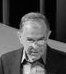
\includegraphics[width=1\hsize]{image200609/bourne.png}
\end{minipage}
\begin{minipage}[t]{0.3\hsize}
   \onslide<1->csh\\
   \onslide<3->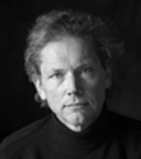
\includegraphics[width=1\hsize]{image200609/billjoy.png} 
\end{minipage}
\begin{minipage}[t]{0.3\hsize}
   \onslide<1->ksh\\
   \onslide<4->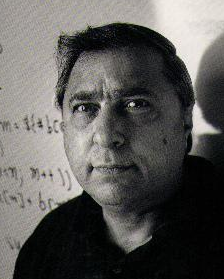
\includegraphics[width=1\hsize]{image200609/korn.png}
\end{minipage}

\begin{center}
    \onslide<5-> Cの普及のための革命必要
\end{center}
\end{frame}

\section{ツール紹介}

\begin{frame}
\frametitle{ツール紹介}

\begin{center}
 \begin{minipage}{0.5\hsize}
 \begin{itemize}
 \item binfmtc
 \item realcsh
 \item realksh
 \end{itemize}
 \end{minipage}
\end{center}

\end{frame}

\subsection{binfmtc}

\begin{frame}
\frametitle{LL化}
\begin{itemize}[<+->]
 \item Cをスクリプト言語みたいに使いたい!
 \item 見た目だけスクリプト言語風
\end{itemize}
\end{frame}

\begin{frame}
\includegraphics[width=0.7\hsize]{image200609/binfmtc.eps}
\end{frame}

\begin{frame}{CをLLっぽく使いたい!}

Linux Kernel の機能を用いてC言語のソースをスクリプトとして実行

{\tt \small
\fbox{\begin{minipage}{1\hsize}
  {\bf coreduo:demo$>$} ./upaccho2.c\\
 upaccho2-webservice.c: In function 'http\_initiate\_webserver':\\
 upaccho2-webservice.c:194: warning: pointer targets in passing argument 3 of 'accept' differ in signedness\\
 Please specify the port as the command-line parameter\\
\end{minipage}}}

\hfill{} \onslide<2->... 一応アプリケーションは動いているがなんだか警告はでている。
\end{frame}

\begin{frame}{CをLLっぽく使いたい!}

修正して即実行

{\tt \small
\fbox{\begin{minipage}{1\hsize}
  {\bf coreduo:demo$>$} ./upaccho2.c\\
 Please specify the port as the command-line parameter\\
\end{minipage}}}

\hfill{} \onslide<2->... なんだかLL!
\end{frame}

\subsection{realcsh}
\begin{frame}
\begin{itemize}[<+->]
 \item C言語をシェルとして使いたい!
 \item cshってあるんだけど、なんか違うよね?
\end{itemize}
\end{frame}

\begin{frame}

{\small \tt 
\fbox{\begin{minipage}{1\hsize}
{\bf coreduo:\~{}$>$} while (1) { printf ( "\%s$\backslash$n", "hello"); }\\
while: Expression Syntax.
\end{minipage}
}}

\hfill{}\onslide<2->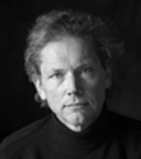
\includegraphics[width=0.3\hsize]{image200609/billjoy.png} 

\end{frame}

\begin{frame}

{\small \tt 
\fbox{\begin{minipage}{1\hsize}
{\bf coreduo:\~{}$>$} realcsh.c\\
{\bf REAL csh:} while (1) { printf ( "\%s$\backslash$n", "hello"); }\\
hello\\
hello\\
hello\\
hello\\
hello\\
.\\
.
\end{minipage}
}}
\end{frame}


\begin{frame}
\includegraphics[width=0.8\hsize]{image200609/realcsh.eps}
\end{frame}

\subsection{realksh}

\begin{frame}
\begin{itemize}[<+->]
 \item C言語はLinux Kernelの開発に利用する言語
 \item コードは試しながら開発したい
 \item シェルが無いと不便だー
 \item そういえば、kshってのがある
\end{itemize}
\end{frame}

\begin{frame}
\frametitle{ksh ってなんで kernel じゃないんだ?}  
\fbox{
\begin{minipage}{0.9\hsize}
{\tt \small
{\bf \$} uname -r \\
2.6.18-rc3dancer\\
{\bf \$} printk ("\%i$\backslash$n", (int) jiffies); \\
ksh: syntax error: `(' unexpected\\
}
\end{minipage}
}

\hfill{}\onslide<2->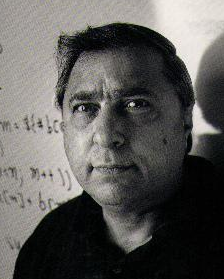
\includegraphics[width=0.3\hsize]{image200609/korn.png}

\end{frame}

\begin{frame}
\frametitle{ksh ってなんで kernel じゃないんだ?}
\fbox{
\begin{minipage}{0.9\hsize}
{\tt \small
{\bf REAL ksh: }$\sharp{}$include $<$linux/utsrelease.h$>$\\
REAL ksh: printk ("\%s$\backslash$n", UTS\_{}RELEASE); \\
  Building modules, stage 2.\\
KMSG: <4>2.6.18-rc3dancer\\
\\
{\bf REAL ksh: }printk ("\%i$\backslash$n", (int) jiffies);\\
  Building modules, stage 2.\\
KMSG: <4>5013786\\

}
\end{minipage}
}

\hfill{}\onslide<2->漢ならこういうシェルがよい
\end{frame}

\begin{frame}
\includegraphics[width=0.7\hsize]{image200609/structure.eps}
\end{frame}

\section{実演}
\begin{frame}
\frametitle{実演}
\begin{itemize}
 \item jiffies の表示
 \item kernel version の表示
 \item BUGの発生
% include <asm/bug.h> BUG()
\end{itemize}
\end{frame}

\section{まとめ}
\begin{frame}
\begin{center}
 \begin{minipage}{0.6\hsize}
 \begin{itemize}[<+->]
 \item LLGONG
 \item Lowlevel Language GONG 
 \item 他のやつらの下をゆけ!
  \item (Debian) \texttt{apt-get install binfmtc} でインストール可能
 \end{itemize}
 \end{minipage}
\end{center}
\end{frame}

\end{document}
